% !TEX TS-program = pdflatex
% !TEX encoding = UTF-8 Unicode

\documentclass{beamer}
% for handouts: \documentclass[handout]{beamer}

%\setbeamertemplate{background canvas}[vertical shading][bottom=white,top=structure.fg!25]
% or whatever

\usetheme[compress]{Amsterdam}
%\setbeamertemplate{headline}{}
%\setbeamertemplate{footline}{}
%\setbeamersize{text margin left=0.5cm}
  
\usepackage[english]{babel}
\usepackage{listings}
\usepackage{geometry}
\usepackage{hyperref}
\usepackage{multicol}



\usepackage{color}

\usepackage[utf8]{inputenc}
\usepackage[T1]{fontenc}
\usepackage{lmodern}

\lstset{
basicstyle=\scriptsize\ttfamily,
columns=flexible,
breaklines=true,
numbers=left,
%stepsize=1,
numberstyle=\tiny,
backgroundcolor=\color[rgb]{0.85,0.90,1}
}


\begin{document}

\title[Automated Content Analysis with Python]{\textbf{Two-day workshop\\ Automated Content Analysis with Python} \\ Day 1}
\author[Damian Trilling]{Damian Trilling \\ ~ \\ \footnotesize{d.c.trilling@uva.nl \\@damian0604} \\ \url{www.damiantrilling.net}}
\date{31-1-2017}
\institute[UvA]{Afdeling Communicatiewetenschap \\Universiteit van Amsterdam}



\begin{frame}{}
\titlepage
\end{frame}

\begin{frame}{Today}
\tableofcontents
\end{frame}



\section[What's ACA?]{What's Automated Content Analysis?}
\begin{frame}[plain]
	What's Automated Content Analysis?
\end{frame}


\begin{frame}[plain]
\begin{figure}
\centering
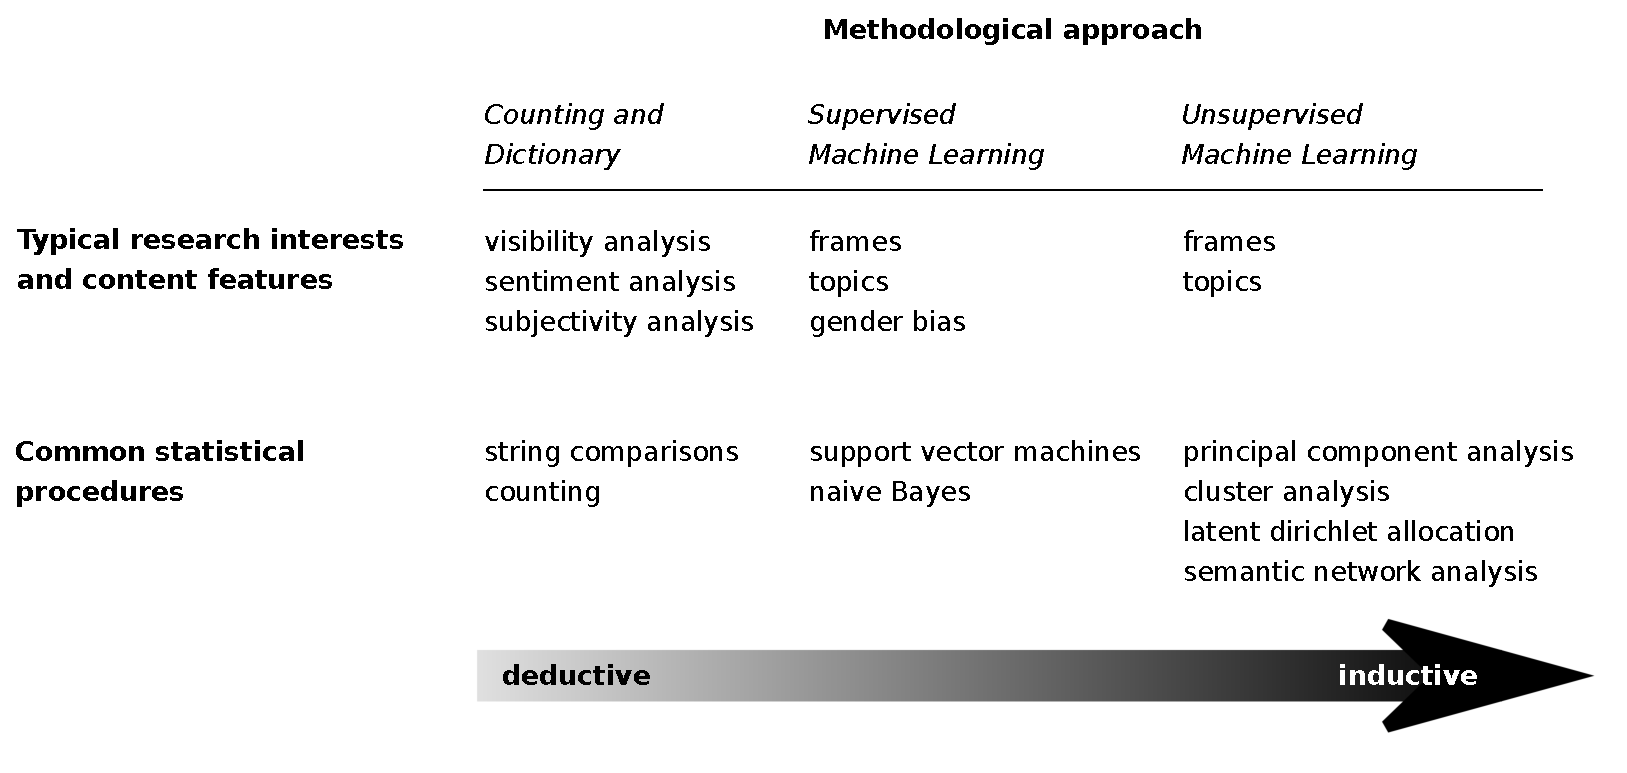
\includegraphics[width=1.0\linewidth]{boumanstrilling2016}
\label{fig:boumanstrilling2016}
\end{figure}
\tiny{Boumans, J. W., \& Trilling, D. (2016). Taking stock of the toolkit: An overview of relevant autmated content analysis approaches and techniques for digital journalism scholars. \emph{Digital Journalism, 4}(1), 8–23. doi:10.1080/21670811.2015.1096598}
\end{frame}


\begin{frame}{Today}
	\begin{itemize}
		\item We'll start with counting/dictionary-based methods
		\item Sentiment analysis
		\item Basic ACA: Natural language processing and regular expressions
		\item<+> But first: A short recap.
	\end{itemize}
	
\end{frame}



\section[Basics]{Recap: The very, very, basics of programming with Python}
\begin{frame}[plain]
\textbf{Recap: The very, very, basics of programming}\\
\vspace{1cm}
You can read all this back in Chapter 4.
\end{frame}
\subsection{Datatypes}


\begin{frame}{Python lingo}
\begin{block}{Basic datatypes (variables)}
\begin{description}
\item[{\color{red}int}] \texttt{32}
\item[{\color{red}float}] \texttt{1.75}
\item[{\color{red}bool}] \texttt{True}, \texttt{False}
\item[{\color{red}string}] \texttt{"Damian"}
\onslide<2->{\scriptsize \item[({\color{red}variable name}] \texttt{firstname})}
\end{description}
\end{block}
\onslide<2->{\textbf{"firstname" and firstname is not the same.\\}}
\onslide<3->{\textbf{"5" and 5 is not the same.}\\ But you can transform it: {\tt{int("5")}} will return 5.}\\
\onslide<3->{\textbf{You cannot calculate \texttt{3 * "5"}} {\tiny{Actually, you can. It gives you "555"}}.\\ But you can calculate {\tt{3 * int("5")}}}
\end{frame}



\begin{frame}{Python lingo}
\begin{block}{More advanced datatypes}
\begin{description}
\item[{\color{red}list}]<2-> \texttt{firstnames = $[$'Damian','Lori','Bjoern'$]$ \\ lastnames = $[$'Trilling','Meester','Burscher'$]$}
\item[{\color{red}list}]<3->\texttt{ages = $[$18,22,45,23$]$}
\item[{\color{red}dict}]<4-> \texttt{familynames= \{'Bjoern': 'Burscher', 'Damian': 'Trilling', 'Lori': 'Meester'\} }
\item[{\color{red}dict}]<4-> \texttt{\{'Bjoern': 26, 'Damian': 31, 'Lori': 25\} }

\end{description}
%Note that the elements of a list, the keys of a dict, and the values of a dict can have any datatype! (It should be consistent, though!)
\end{block}
\end{frame}



\begin{frame}{Python lingo}
\begin{block}{Functions}
\begin{description}
\item[{\color{red}functions}]<2-> Take an input and return something else \\ {\tt{int(32.43})} returns the integer 32. \texttt{len("Hello")} returns the integer 5.\\ 
\item[{\color{red}methods}]<3-> are similar to functions, but directly associated with an object. {\tt{"SCREAM".lower()}} returns the string "scream"
\end{description}
\end{block}
\onslide<4->{Both functions and methods end with \texttt{()}. Between the \texttt{()}, \emph{arguments} can (sometimes have to) be supplied.}
\end{frame}


\subsection[Indention]{Indention: The Python way of structuring your program}
\begin{frame}[plain]
Indention: The Python way of structuring your program
\end{frame}


\begin{frame}[fragile]{Indention}
\begin{block}{Structure}
The program is structured by TABs or SPACEs
\end{block}

\end{frame}



{\setbeamercolor{background canvas}{bg=black}
\begin{frame}[plain]
\makebox[\linewidth]{
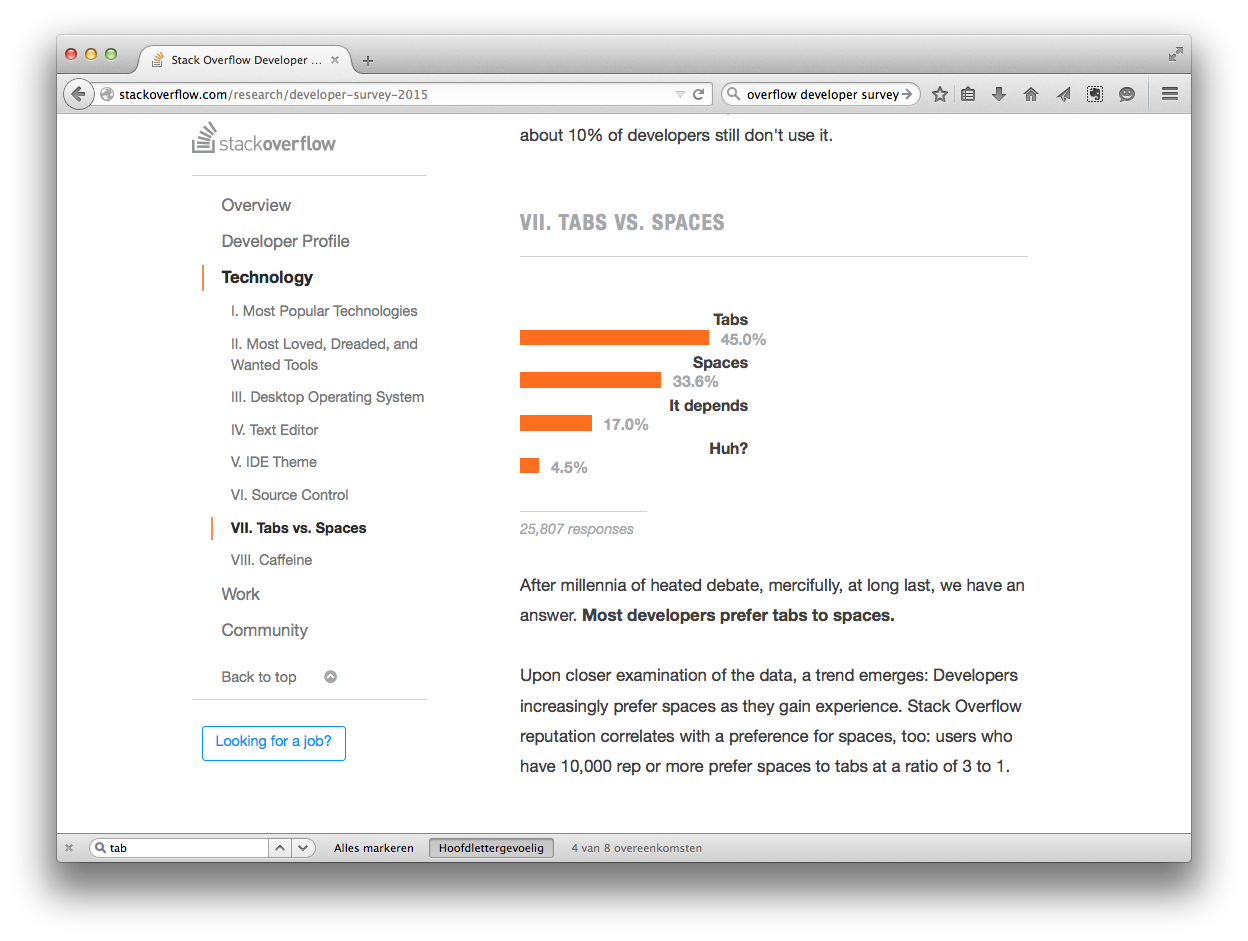
\includegraphics[width=\paperwidth,height=\paperheight,keepaspectratio]{tabsvsspaces}
}
\end{frame}
}

\begin{frame}[fragile]{Indention}
\begin{block}{Structure}
The program is structured by TABs or SPACEs
\end{block}
\begin{lstlisting}
firstnames=['Damian','Lori','Bjoern']
age={'Bjoern': 27, 'Damian': 32, 'Lori': 26}
print ("The names and ages of all BigData people:")
for naam in firstnames:
    print (naam,age[naam])
\end{lstlisting}
\onslide<2->{\textbf{Don't mix up TABs and spaces! Both are valid, but you have to be consequent!!! Best: always use 4 spaces!}}
\end{frame}





\begin{frame}[fragile]{Indention}
\begin{block}{Structure}
The program is structured by TABs or SPACEs
\end{block}
\begin{lstlisting}
print ("The names and ages of all BigData people:")
for naam in firstnames:
    print (naam,age[naam])
    if naam=="Damian":
        print ("He teaches this course")
    elif naam=="Lori":
        print ("She was an assistant last year")
    elif naam=="Bjoern":
        print ("He helps on Wednesdays")
    else:
        print ("No idea who this is")
\end{lstlisting}
\end{frame}


\begin{frame}{Indention}
The line \emph{before} an indented block starts with a \emph{statement} indicating what should be done with the block and ends with a \texttt{:}

\begin{block}{Indention of the block indicates that}<2->
\begin{itemize}
\item<3-> it is to be executed repeatedly (\texttt{for} statement) – e.g., for each element from a list
\item<4-> it is only to be executed under specific conditions (\texttt{if}, \texttt{elif}, and \texttt{else} statements)
\item<5-> an alternative block should be executed if an error occurs (\texttt{try} and \texttt{except} statements)
\item<6-> a file is opened, but should be closed again after the block has been executed (\texttt{with} statement)
\end{itemize}
\end{block}
\end{frame}



\begin{frame}[plain]
Exercise
\end{frame}



\section{Sentiment Analysis}
\begin{frame}
Sentiment analysis
\end{frame}




\begin{frame}{What is sentiment analysis?}
	\begin{block}{Extracting subjective information from texts}
		\begin{itemize}
			\item<2->  the author's attitude towards the topic of the text
			\item<3-> \emph{polarity}: negative---positive
			\item<4-> \emph{subjectivity}: neutral---subjective *
			\item<5-> advanced approaches: different emotions
		\end{itemize}
		~\\ 
		\footnotesize{
			\onslide<6->{* Less sophisticated approaches do not see this as a sperate dimension but simply calculate $objectivity=1-(negativity+positivity)$}}
	\end{block}
\end{frame}

%
%
%\begin{frame}{Applications}
%	\begin{block}{Who uses it?}
%		\begin{itemize}
%			\item Companies
%			\item especially for Web Analytics
%			\item Social Scientists
%			\item applications in data journalism, politics, \ldots
%		\end{itemize}
%		Many references to examples in Mostafa (2013).
%	\end{block}
%	~\\
%	$\Rightarrow$ Cases in which you have a huge amount of data or real-time data and you want to get an idea of the tone. \\ ~
%	\par
%	\tiny{Mostafa, M. M. (2013). More than words: Social networks’ text mining for consumer brand sentiments. \emph{Expert Systems with Applications, 40}(10), 4241– 4251. doi:10.1016/j.eswa.2013.01.019}\\
%\end{frame}


\begin{frame}[fragile]{Example}
\begin{lstlisting}
>>> sentiment("Great service by @NSHighspeed")
(0.8, 0.75)
>>> sentiment("Bad  service by @NSHighspeed")
(-0.6166666666666667, 0.6666666666666666)
\end{lstlisting}
	~\\
	\footnotesize{(polarity, subjectivity) with \\ ~ \\
		$-1 \leq polarity \leq +1$\\
		$0 \leq subjectivity \leq +1$ )} \\~\\
	\tiny{This is the module pattern.nl, available for Python 2 only. \\ De Smedt, T., \& Daelemans W. (2012).  Pattern for Python. \emph{Journal of Machine Learning Research, 13}, 2063-2067.\\}
\end{frame}

\subsection{Bag-of-words approaches}

\begin{frame}{Bag-of-words approaches}
	\begin{block}{How does it work?}
		\begin{itemize}
			\item We take each word of a text and look if it's positive or negative.
			\begin{itemize}
				\item<2-> Most simple way: compare it with a list of negative words and with a list of positive words %{\small(That's what Mostafa (2013) did)}
				\item<3-> More advanced: look up a subjectivity score from a table 
			\end{itemize}
			\item<4-> e.g., add up the scores and average them.
		\end{itemize}
	\end{block}
\end{frame}

%
%\begin{frame}[fragile]{How to do this}
%	If you were to run an analyis like the one by Mostafa (2013), how could you do this?
%\end{frame}

\begin{frame}[fragile]{How to do this}
\scriptsize{ 
	(given a \emph{string} \texttt{tekst} that you want to analyze and two 
	\emph{lists} of strings with negative and positive words, 
	\texttt{lijstpos=$[$"great","fantastic",\ldots,"perfect"$]$} and \texttt{lijstneg})\\
}

\begin{lstlisting}
sentiment=0
for woord in tekst.split():
    if woord in lijstpos:
        sentiment=sentiment+1    #same as sentiment+=1
    elif woord in lijstneg:
        sentiment=sentiment-1    #same as sentiment-=1
print (sentiment)
\end{lstlisting}
%if sentiment > 0:
%    print "This was a positive text".
%elif sentiment < 0:
%    print "This was a negative text".    
%elif sentiment == 0:
%    print "We could not identify any tendency".    
\end{frame}


\begin{frame}[fragile]{Do we need to have the lists in our program itself?}
No.\\
You could have them in a separate text file, one per row, and then read that file directly to a list.\\
\begin{lstlisting}
poslijst=open("filewithonepositivewordperline.txt").read().splitlines()
neglijst=open("filewithonenegativewordperline.txt").read().splitlines()
\end{lstlisting}
\end{frame}


{\setbeamercolor{background canvas}{bg=black}
	\begin{frame}[plain]
		\makebox[\linewidth]{
			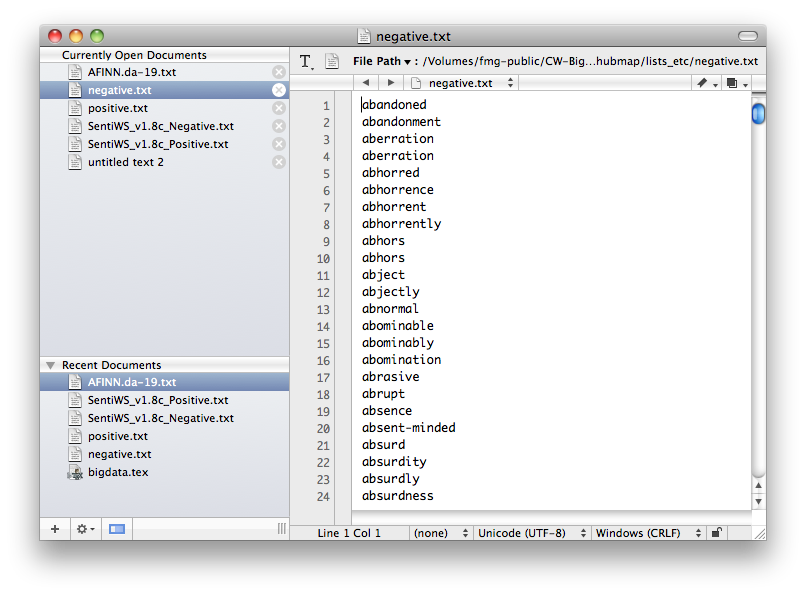
\includegraphics[width=\paperwidth,height=\paperheight,keepaspectratio]{woordenlijst1.png}}
	\end{frame}
}


\begin{frame}{More advanced versions}
	\begin{itemize}
		\item CSV files or similar tables with weights
		\item Or some kind of dict?
	\end{itemize}
\end{frame}

{\setbeamercolor{background canvas}{bg=black}
	\begin{frame}[plain]
		\makebox[\linewidth]{
			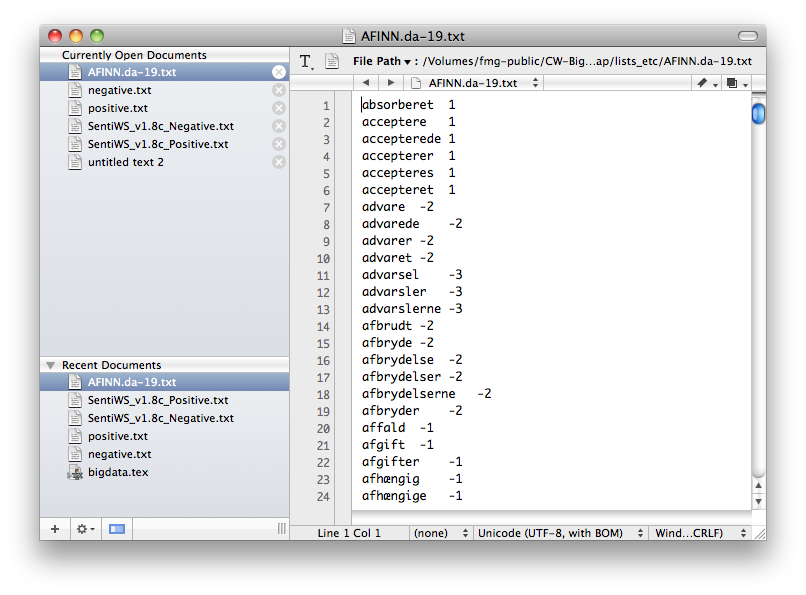
\includegraphics[width=\paperwidth,height=\paperheight,keepaspectratio]{woordenlijst2.png}}
	\end{frame}
	\begin{frame}[plain]
		\makebox[\linewidth]{
			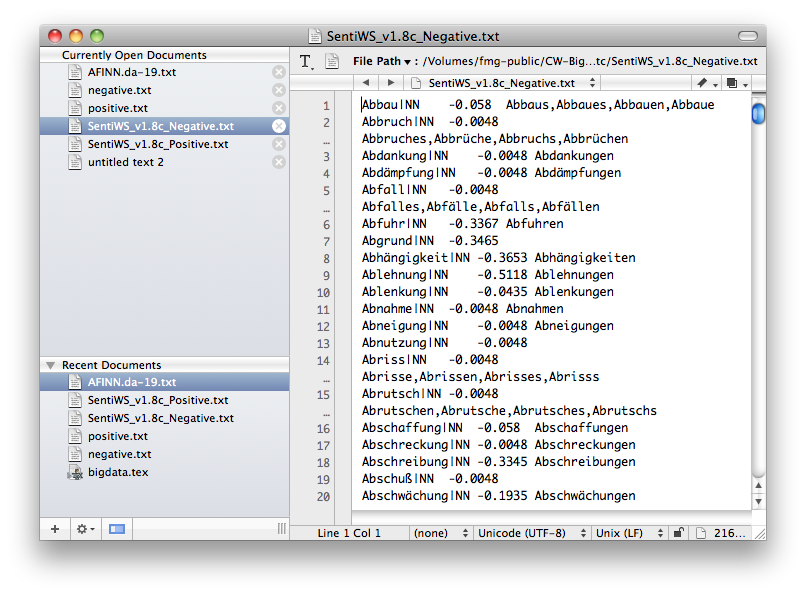
\includegraphics[width=\paperwidth,height=\paperheight,keepaspectratio]{woordenlijst3.png}}
	\end{frame}
}

%
%
%\begin{frame}{Mustafa 2013: Interpreting the output}
%	
%	\begin{columns}
%		\column{.7\textwidth}
%		\makebox[\columnwidth]{
%			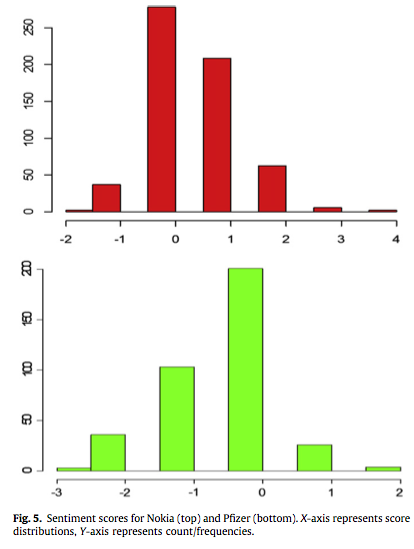
\includegraphics[width=\paperwidth,height=.7\paperheight,keepaspectratio]{plaatje_uit_mostafa2013.png}
%		}
%		\column{.3\textwidth}
%		\onslide<2->{Your thoughts?}
%		\onslide<3->{
%			\begin{itemize}
%				\item each word counts equally (1)
%				\item many tweets contain no words from the list. What does this mean?
%				\item Ways to improve BOW approaches?
%			\end{itemize}
%		}
%	\end{columns}
%\end{frame}

% nog iets met die scores. dus een beter voorbeeld. Een tweede


\begin{frame}{Bag-of-words approaches}
	\begin{block}{pro}<2->
		\begin{itemize}
			\item easy to implement
			\item easy to modify:
			\begin{itemize}
				\item add or remove words
				\item make new lists for other languages, other categories (than positive/negative), \dots
			\end{itemize}
			\item easy to understand (transparency, reproducability)
		\end{itemize}
	\end{block}
	\par
	\tiny{e.g., Schut, L. (2013). Verenigde Staten vs. Verenigd Koningrijk: Een automatische inhoudsanalyse naar verklarende factoren voor het gebruik van positive campaigning en negative campaigning door vooraanstaande politici en politieke partijen op Twitter. \emph{Bachelor Thesis}, Universiteit van Amsterdam.}\\
\end{frame}



\begin{frame}{Bag-of-words approaches}
	\begin{block}{con}
		\begin{itemize}
			\item simplistic assumptions
			\item e.g., intensifiers cannot be interpreted ("really" in "really good" or "really bad")
			\item or, even more important, negations.
		\end{itemize}
	\end{block}
\end{frame}



\subsection{Advanced approaches}
\begin{frame}
	Sentiment analysis:\\
	Advanced approaches
\end{frame}


\begin{frame}{Improving the BOW approach}
	\begin{block}{Example: The Sentistrenght algorithm}
		\begin{itemize}
			\item $-5\ldots-1$ and $+1\ldots+5$
			\item spelling correction
			\item "booster word list" for strengthening/weakening the effect of the following word
			\item interpreting repeated letters ("baaaaaad"), CAPITALS and !!!
			\item idioms
			\item negation 
			\item ldots
		\end{itemize}
	\end{block}
	~ \\
	\tiny{Thelwall, M., Buckley, K., \& Paltoglou, G. (2012). Sentiment strength detection for the social Web. \emph{Journal of the American Society for Information Science and Technology, 63}(1), 163-173.\\}
\end{frame}


\begin{frame}{Advanced approaches}
	\begin{block}{Take the structure of a text into account}
		\begin{itemize}
			\item Try to apply linguistics concepts to identify sentence structure
			\item can identify negations
			\item can interpret intensifiers
		\end{itemize}
	\end{block}
\end{frame}


\begin{frame}[fragile]{Example}
\begin{lstlisting}
from pattern.nl import sentiment
>>> sentiment("Great service by @NSHighspeed")
(0.8, 0.75)
>>> sentiment("Really")
(0.0, 1.0)
>>> sentiment("Really Great service by @NSHighspeed")
(1.0, 1.0)
\end{lstlisting}
~\\
\footnotesize{(polarity, subjectivity) with \\
	$-1 \leq polarity \leq +1$\\
	$0 \leq subjectivity \leq +1$ )\\} ~ \\
Unlike in pure bag-of-words approaches, here, the overall sentiment is not just the sum or the average of its parts! \\
\tiny{De Smedt, T., \& Daelemans W. (2012).  Pattern for Python. \emph{Journal of Machine Learning Research, 13}, 2063-2067.}
\end{frame}




\begin{frame}{Advanced approaches}
	\begin{block}{pro}<2->
		\begin{itemize}
			\item understand intensifiers or negation
			\item thus: higher accuracy
		\end{itemize}
	\end{block}
	\begin{block}{con}<3->
		\begin{itemize}
			\item Black box? Or do we understand the algorithm?
			\item Difficult to adapt to own needs
			\item \emph{really} much better results?
		\end{itemize}
	\end{block}
\end{frame}

%
%
%\subsection{A sentiment analysis tailored to your needs!}
%\begin{frame}
%	Data analysis 1: Sentiment analysis\\
%	A sentiment analysis tailored to your needs!
%\end{frame}
%
%
%
%
%\begin{frame}{A sentiment analysis tailored to your needs!}
%	\begin{block}{Identifying suicidal texts}
%		\begin{itemize}
%			\item Bag-of-words-approach with very specific dictionary
%			\item added negation
%			\item added regular expression search for key phrases
%			\item Very specific design requirements: False positives are OK, false negatives not!
%		\end{itemize}
%	\end{block}
%	\par
%	\tiny{Huang, Y.-P., Goh, T., \& Liew, C.L. (2007). Hunting suicide notes in web 2.0 – preliminary findings. \emph{Ninth IEEE International Symposium on Multimedia}. Retrieved from http://ieeexplore.ieee.org/stamp/stamp.jsp?tp=\&arnumber=4476021}\\
%\end{frame}
%
%\begin{frame}{}
%	Already this still relatively simple approach seems to work satisfactory, but if 106 scientists from 24 competing teams (!) work on it, they can 
%	\begin{block}{group suidide notes by these characteristics:}<2->
%		\begin{multicols}{2}
%			{\small {
%					\begin{itemize}
%						\item swear
%						\item family
%						\item friend
%						\item positive emotion
%						\item negative emotion
%						\item anxiety
%						\item anger
%						\item sad
%						\item cognitive process
%						\item biology
%						\item sexual
%						\item ingestion
%						\item religion
%						\item death
%					\end{itemize}
%				}}
%			\end{multicols}
%		\end{block}
%		\par
%		\tiny{Pestian, J.P.; Matykiewicz, P., Linn-Gust, M., South, B., Uzuner, O., Wiebe, J., Cohen, K.B., Hurdle, J., \& Brew, C. (2012). Sentiment analysis of suicide notes: A shared task. \emph{Biomedical Informatics Insights, 5}(1), p. 3-16. Retrieved from http://europepmc.org/articles/PMC3299408?pdf=render}\\
%	\end{frame}
%	
%	
%	\begin{frame}{Sidenote}
%		An alternative state-of-the-art approach:
%		\begin{block}{Use supervised machine learning}
%			\begin{itemize}
%				\item Instead of defining rules, hand-code (``annotate'') the sentiment of some tweets manually and let the computer find out which words or characters (``features'') predict sentiment
%				\item Then use this model to predict sentiment for other tweets
%				\item Essentially the same like what you know since the second year of your Bachelor: regression analysis (but now with DV sentiment and IV's word occurrences)
%				\item $\Rightarrow$ week 8
%			\end{itemize}
%			\tiny{Gonzalez-Bailon, S., \& Paltoglou, G. (2015). Signals of public opinion in online communication: A comparison of methods and data sources. \emph{The ANNALS of the American Academy of Political and Social Science, 659}(1), 95-–107.}
%		\end{block}
%		
%	\end{frame}
%	
	



\begin{frame}[plain]
Exercise
\end{frame}





\section[Basic ACA]{Basic ACA: Dictionary- and string-based methods}





\subsection[Stopword removal]{Stopword removal}

\subsection{Natural language processing}
\begin{frame}{Stopword removal: What and why?}
	\begin{block}{Why remove stopwords?}
		\begin{itemize}
			\item If we want to identify key terms (e.g., by means of a word count), we are not interested in them
			\item If we want to calculate document similarity, it might be inflated
			\item If we want to make a word co-occurance graph, irrelevant information will dominate the picture
		\end{itemize}
	\end{block}
\end{frame}

\subsection{A simple algorithm}

\begin{frame}[fragile]{Stopword removal: How}
\begin{lstlisting}
testo='He gives her a beer and a cigarette.'
testonuovo=""
stopwords=['and','the','a','or','he','she','him','her']
for verbo in testo.split():
    if verbo not in stopwords:
        testonuovo=testonuovo+verbo+" "
\end{lstlisting}
What do we get if we do:
\begin{lstlisting}
print (testonuovo)
\end{lstlisting}
Can you explain the algorithm?
\end{frame}




\begin{frame}[fragile]{We get:}
\begin{lstlisting}
>>> print  (testonuovo)
'He gives beer cigarette. '
\end{lstlisting}
Why is "He" still in there? \\ How can we fix this?
\end{frame}

\begin{frame}[fragile]{Stopword removal}
\begin{lstlisting}
testo='He gives her a beer and a cigarette.'
testonuovo=""
stopwords=['and','the','a','or','he','she','him','her']
    for verbo in testo.split():
        if verbo.lower() not in stopwords:
        testonuovo=testonuovo+verbo+" "
\end{lstlisting}
\end{frame}










\subsection{Regular expressions}

\begin{frame}
Automated content analysis using regular expressions
\end{frame}

\begin{frame}{Regular Expressions: What and why?}
\begin{block}{What is a regexp?}
\begin{itemize}
\item<1-> a \emph{very} widespread way to describe patterns in strings
\item<2-> Think of wildcards like {\tt{*}} or operators like {\tt{OR}}, {\tt{AND}} or {\tt{NOT}} in search strings: a regexp does the same, but is \emph{much} more powerful
\item<3-> You can use them in many editors (!), in the Terminal, in STATA \ldots and in Python
\end{itemize}
\end{block}
\end{frame}

\begin{frame}{An example}
\begin{block}{From last week's task}
\begin{itemize}
\item We wanted to remove everything but words from a tweet
\item We did so by calling the \texttt{.replace()} method
\item We could do this with a regular expression as well: \\
{\tt{ \lbrack \^{}a-zA-Z\rbrack}} would match anything that is not a letter
\end{itemize}
\end{block}
\end{frame}

\begin{frame}{Basic regexp elements}
\begin{block}{Alternatives}
\begin{description}
\item[{\tt{\lbrack TtFf\rbrack}}] matches either T or t or F or f
\item[{\tt{Twitter|Facebook}}] matches either Twitter or Facebook
\item[{\tt{.}}] matches any character
\end{description}
\end{block}
\begin{block}{Repetition}<2->
\begin{description}
\item[{\tt{*}}] the expression before occurs 0 or more times
\item[{\tt{+}}] the expression before occurs 1 or more times
\end{description}
\end{block}
\end{frame}

\begin{frame}{regexp quizz}
\begin{block}{Which words would be matched?}
\tt
\begin{enumerate}
\item<1-> \lbrack Pp\rbrack ython
\item<2-> \lbrack A-Z\rbrack +
\item<3-> RT :* @\lbrack a-zA-Z0-9\rbrack *
\end{enumerate}
\end{block}
\end{frame}

\begin{frame}{What else is possible?}
If you google {\tt{regexp}} or {\tt{regular expression}}, you'll get a bunch of useful overviews. The wikipedia page is not too bad, either. 
\end{frame}

\begin{frame}{How to use regular expressions in Python}
\begin{block}{The module re}
\begin{description}
\item<1->[{\tt{re.findall("\lbrack Tt\rbrack witter|\lbrack Ff\rbrack acebook",testo)}}] returns a list with all occurances of Twitter or Facebook in the string called {\tt{testo}}
\item<1->[{\tt{re.findall("\lbrack 0-9\rbrack +\lbrack a-zA-Z\rbrack +",testo)}}] returns a list with all words that start with one or more numbers followed by one or more letters in the string called {\tt{testo}}
\item<2->[{\tt{re.sub("\lbrack Tt\rbrack witter|\lbrack Ff\rbrack acebook","a social medium",testo)}}] returns a string in which all all occurances of Twitter or Facebook are replaced by "a social medium"
\end{description}
\end{block}
\end{frame}


\begin{frame}[fragile]{How to use regular expressions in Python}
\begin{block}{The module re}
\begin{description}
\item<1->[{\tt{re.match(" +(\lbrack 0-9\rbrack +) of (\lbrack 0-9\rbrack +) points",line)}}] returns  \texttt{None} unless it \emph{exactly} matches the string \texttt{line}. If it does, you can access the part between () with the \texttt{.group()} method.
\end{description}
\end{block}

Example:
\begin{lstlisting}
line="             2 of 25 points"
result=re.match(" +([0-9]+) of ([0-9]+) points",line)
if result:
   print ("Your points:",result.group(1))
   print ("Maximum points:",result.group(2))
\end{lstlisting}
Your points: 2\\
Maximum points: 25
\end{frame}














\begin{frame}{Possible applications}
\begin{block}{Data preprocessing}
\begin{itemize}
\item Remove unwanted characters, words, \ldots
\item Identify \emph{meaningful} bits of text: usernames, headlines, where an article starts, \ldots
\item filter (distinguish relevant from irrelevant cases)
\end{itemize}
\end{block}
\end{frame}


\begin{frame}{Possible applications}
\begin{block}{Data analysis: Automated coding}
\begin{itemize}
\item Actors
\item Brands
\item links or other markers that follow a regular pattern
\item Numbers (!)
\end{itemize}
\end{block}
\end{frame}

\begin{frame}[fragile,plain]{Example 1: Counting actors}
\begin{lstlisting}
import re, csv
from os import listdir, path
mypath ="/home/damian/artikelen"
filename_list=[]
matchcount54_list=[]
matchcount10_list=[]
onlyfiles = [f for f in listdir(mypath) if path.isfile(path.join(mypath,f))]
for f in onlyfiles:
   matchcount54=0
   matchcount10=0
   with open(path.join(mypath,f),mode="r",encoding="utf-8") as fi:
      artikel=fi.readlines()
      for line in artikel:
         matches54 = re.findall('Israel.*(minister|politician.*|[Aa]uthorit)',line)
         matches10 = re.findall('[Pp]alest',line)         
         matchcount54+=len(matches54)
         matchcount10+=len(matches10)
      filename_list.append(f)
      matchcount54_list.append(matchcount54)
      matchcount10_list.append(matchcount10)
output=zip(filename_list,matchcount10_list,matchcount54_list)
with open("overzichtstabel.csv", mode='w',encoding="utf-8") as fo:
    writer = csv.writer(fo)
    writer.writerows(output)
\end{lstlisting}
\end{frame}




\begin{frame}[fragile]{Example 2: Which number has this Lexis Nexis article?}
\begin{lstlisting}
                              All Rights Reserved

                               2 of 200 DOCUMENTS

                                  De Telegraaf

                             21 maart 2014 vrijdag

Brussel bereikt akkoord  aanpak probleembanken;
ECB krijgt meer in melk te brokkelen

SECTION: Finance; Blz. 24
LENGTH: 660 woorden

BRUSSEL   Europa heeft gisteren op de valreep een akkoord bereikt 
over een saneringsfonds voor banken. Daarmee staat de laatste
\end{lstlisting}

\end{frame}

\begin{frame}[fragile]{Example 2: Check the number of a lexis nexis article}
\begin{lstlisting}
                              All Rights Reserved

                               2 of 200 DOCUMENTS

                                  De Telegraaf

                             21 maart 2014 vrijdag

Brussel bereikt akkoord  aanpak probleembanken;
ECB krijgt meer in melk te brokkelen

SECTION: Finance; Blz. 24
LENGTH: 660 woorden

BRUSSEL   Europa heeft gisteren op de valreep een akkoord bereikt 
over een saneringsfonds voor banken. Daarmee staat de laatste
\end{lstlisting}

\begin{lstlisting}
for line in tekst:
    matchObj=re.match(r" +([0-9]+) of ([0-9]+) DOCUMENTS",line)
    if matchObj:
        numberofarticle= int(matchObj.group(1))
        totalnumberofarticles= int(matchObj.group(2))
\end{lstlisting}
\end{frame}


\begin{frame}{Practice yourself!}
\huge{\url{http://www.pyregex.com/}}
\end{frame}

\subsection{Some more Natural Language Processing}
\begin{frame}
Some more Natural Language Processing
\end{frame}



\begin{frame}{Some more NLP: What and why?}
\begin{block}{What can we do?}
\begin{itemize}
\item<1-> remove stopwords \emph{(last week)}
\item<2-> stemming
\item<3-> Parse sentences (advanced)
\end{itemize}
\end{block}
\end{frame}

\begin{frame}{NLP: What and why?}
\begin{block}{Why do stemming?}
\begin{itemize}
\item Because we do not want to distinguish between smoke, smoked, smoking, \ldots
\item Typical preprocessing step (like stopword removal)
\end{itemize}
\end{block}
\end{frame}

\begin{frame}[fragile]{Stemming}
{\footnotesize{(with NLTK, see Bird, S., Loper, E., \& Klein, E. (2009). \emph{Natural language processing with Python}. Sebastopol, CA: O’Reilly.)}}
\begin{lstlisting}
from nltk.stem.snowball import SnowballStemmer
stemmer=SnowballStemmer("english")
frase="I am running while generously greeting my neighbors"
frasenuevo=""
for palabra in frase.split():
    frasenuevo=frasenuevo + stemmer.stem(palabra)  + " "
\end{lstlisting}
If we now did {\tt{print(frasenuevo)}}, it would return:
\begin{lstlisting}
i am run while generous greet my neighbor
\end{lstlisting}
\end{frame}

\begin{frame}[fragile]{Stemming and stopword removal - let's combine them!}
\begin{lstlisting}
from nltk.stem.snowball import SnowballStemmer
from nltk.corpus import stopwords
stemmer=SnowballStemmer("english")
stopwords = stopwords.words("english")
frase="I am running while generously greeting my neighbors"
frasenuevo=""
for palabra in frase.lower().split():
    if palabra not in stopwords:
        frasenuevo=frasenuevo + stemmer.stem(palabra)  + " "
\end{lstlisting}
Now, {\tt{print(frasenuevo)}} returns:
\begin{lstlisting}
run generous greet neighbor
\end{lstlisting}
Perfect!\\
\onslide<2>{
\tiny{In order to use \texttt{nltk.corpus.stopwords}, you have to download that module once. You can do so by typing the following in the Python console and selecting the appropriate package from the menu that pops up: \\ \texttt{import nltk\\nltk.download()}\\NB: Don't download everything, that's several GB.\\}}
\end{frame}

{\setbeamercolor{background canvas}{bg=black}
\begin{frame}[plain]
\makebox[\linewidth]{
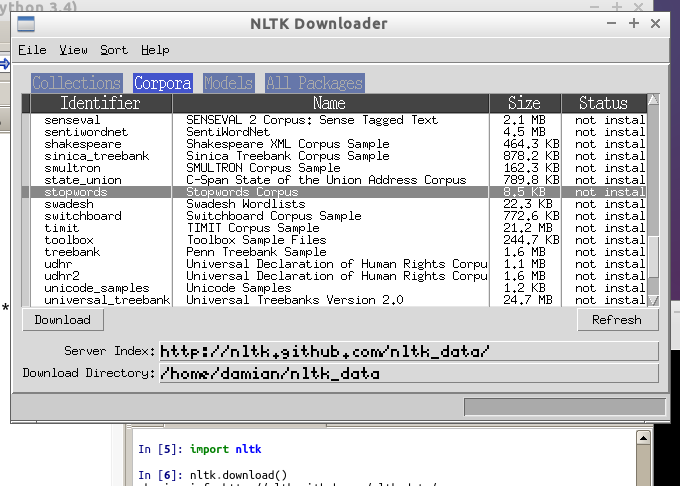
\includegraphics[width=\paperwidth,height=\paperheight,keepaspectratio]{nltk-download.png}}
\end{frame}
}



\begin{frame}{NLP: What and why?}
\begin{block}{Why parse sentences?}
\begin{itemize}
\item To find out what grammatical function words have
\item and to get closer to the meaning.
\end{itemize}
\end{block}
\end{frame}

\begin{frame}[fragile]{Parsing a sentence}
\begin{lstlisting}
import nltk
sentence = "At eight o'clock on Thursday morning, Arthur didn't feel very good."
tokens = nltk.word_tokenize(sentence)
print (tokens)
\end{lstlisting}

\texttt{nltk.word\_tokenize(sentence)} is similar to sentence.split(), but compare handling of punctuation and the \texttt{didn't} in the output:
\begin{lstlisting}
['At', 'eight', "o'clock", 'on', 'Thursday', 'morning','Arthur', 'did', "n't", 'feel', 'very', 'good', '.']
\end{lstlisting}
\end{frame}


\begin{frame}[fragile]{Parsing a sentence}
Now, as the next step, you can ``tag'' the tokenized sentence:
\begin{lstlisting}
tagged = nltk.pos_tag(tokens)
print (tagged[0:6])
\end{lstlisting}
gives you the following:
\begin{lstlisting}
[('At', 'IN'), ('eight', 'CD'), ("o'clock", 'JJ'), ('on', 'IN'),
('Thursday', 'NNP'), ('morning', 'NN')]
\end{lstlisting}

\onslide<2->{
And you could get the word type of "morning" with \texttt{tagged[5][1]}!
}

\end{frame}


\begin{frame}{More NLP}
\Huge{Look at \url{http://nltk.org}}

\end{frame}





\begin{frame}[plain]
Exercise
\end{frame}












\end{document}


